%
% tkz-euclide (14/01/2011)
%
% Coding (utf8) Creator (TeX) Producer (pdfeTeX) 
% Author Alain Matthes
\input{tkzfctpreamble.ltx}

\begin{document}

\begin{tikzpicture}[scale=2]
  \tikzstyle{tan style}=[-]
  \tkzInit[xmin=-5,xmax=2,ymin=-1,ymax=3]
  \tkzDrawXY
  \tkzText[draw,color = red, fill = orange!20](1.5,1.5){$y = xe^x$}
  \global\edef\tkzFctLast{x*exp(x)}% c'est la ligne importante
  \foreach \v in {-4,-3.8,...,0}{%
    \tkzDrawTangentLine[color=blue,line width=.4pt,kl=1](\v)}
  \foreach \v in {0.6,0.8,1}{%
    \tkzDrawTangentLine[color=blue,line width=.4pt,kr=0,kl=.75](\v)}
\end{tikzpicture}

\end{document} 
